\section{Experiments}
\label{sec:exp}

We demonstrate the effectiveness of \headname{} as a pre-execution auditor for a frozen driving VLA.
In \cref{sec:res-signal}, we show that the frozen last token carries a scene-specific audit signal and that the signal is causal.
In \cref{sec:res-onetoken}, we show that reading the full prefill sequence is worse than reading its last token.
In \cref{sec:res-incumbent,sec:res-selloss}, we report an adequately powered comparison against a trained trajectory-geometry auditor and the controlled effect of the selector loss.
In \cref{sec:res-eff}, we report deployment cost.
All numbers are computed once from hash-locked predictions and read directly from the locked analysis records; \cref{tab:main-abs} reports absolute levels, and \cref{tab:main} and \cref{fig:results} summarize every primary contrast.

The generator is \vlaname{} (10B), frozen throughout.
For each decision group it samples $K{=}8$ candidates from one prompt prefill of 3{,}086 tokens; the final-layer hidden states are captured in the same call (\cref{sec:capture}).
The \headname{} head has 1{,}708{,}871 trainable parameters, is trained with AdamW under 5-fold scene-level cross-validation with three seeds, and selects checkpoints on inner validation only.
All arms share the identical graph and parameter count.
Endpoints are computed at $K{=}8$ (co-primary) and $K{=}2/5$ (secondary), aggregated group to scene to seed, with paired scene bootstrap intervals over $10{,}000$ resamples.

\subsection{Setup}
\label{sec:setup}

Scenes advance through four rungs (\cref{tab:ladder}).
Development scenes absorbed all architecture and objective design, including every repair and failed branch.
The prospective untouched cohort (173 scenes, 519 groups, 4{,}152 candidate scores) was frozen outcome-blind, that is, captured, hashed, and quarantined before any model consumed it, and first opened by the confirmatory matched-visibility study of \cref{sec:res-signal,sec:res-onetoken}.
The extension cohort (352 additional scenes) exists solely to power the incumbent study of \cref{sec:res-incumbent}.
A sealed 35-scene cohort is opened only if an auditor is promoted; it was not.

\begin{table}[t]
  \centering
  \small
  \setlength{\tabcolsep}{4pt}
  \begin{tabular}{@{}llll@{}}
    \toprule
    Rung & Scenes & Role & Status \\
    \midrule
    Development & 122 & design, repairs & opened freely \\
    Prospective & 173 & confirmatory M-study & used once \\
    Extension & +352 & powered N-study & used once \\
    Sealed & 35 & one-shot confirmation & never opened \\
    \bottomrule
  \end{tabular}
  \caption{\textbf{Cohort ladder.} Each rung is hash-frozen before use.}
  \label{tab:ladder}
\end{table}

The endpoints are selected regret and tie-aware top-1 agreement at $K{=}8$, as defined in \cref{sec:setting}.
Selected regret is exactly the slack that minADE@$K$-style reporting hides: the gap between the best available candidate's outcome and the outcome of the candidate the deployed rule commits to.
We report both because they can disagree: an auditor can commit to near-best candidates reliably (low regret) while losing top-1 agreement, and vice versa; \cref{sec:res-incumbent} shows precisely this tension.

We compare four auditors, trained on identical labels and folds.
\Ltok{} reads the last prefill token $h$.
\Lfull{} reads the full sequence $H$ (parameter-matched to \Ltok{}, interchangeable state dicts).
\Lnull{} is the matched scene-blind control: the scene input is a single zero token with no learned null embedding, so the arm retains the identical graph and capacity but no scene information.
\Lgeo{} is the trained incumbent, a trajectory-geometry-only MLP (about 202k parameters, its own frozen objective) that sees no VLA representation at all.
The matched-visibility study compares
M1 $=$ \Lfull$-$\Ltok,
M2 $=$ \Lfull$-$\Lnull,
M3 $=$ \Ltok$-$\Lnull,
M4 $=$ \Lfull$-$\Lgeo, and
M5 $=$ \Ltok$-$\Lgeo{}
(paired per scene, three seeds each).

\begin{table}[t]
  \centering
  \small
  \begin{tabular}{@{}lccc@{}}
    \toprule
    Arm & Regret $\downarrow$ & Top-1 $\uparrow$ & Pairwise $\uparrow$ \\
    \midrule
    \Lnull{} (scene-blind) & $0.0439$ & $0.567$ & $0.741$ \\
    \Lgeo{} (incumbent) & $0.0422$ & $0.700$ & $0.827$ \\
    \Lfull{} (sequence) & $0.0456$ & $0.614$ & $0.776$ \\
    \Ltok{} (ours) & $\mathbf{0.0371}$ & $0.667$ & $0.809$ \\
    \bottomrule
  \end{tabular}
  \caption{\textbf{Absolute levels on the prospective untouched cohort} (173 scenes, 519 groups, three seeds; scene-macro means @$K{=}8$). Bold marks the best regret.}
  \label{tab:main-abs}
\end{table}

Causal ablations run on the representation-reading arm, at inference time and with the training entirely untouched:
\textsc{wrong-scene} substitutes the representation of a different scene under a preregistered donor mapping;
\textsc{zero} zeroes the representation;
a \textsc{last-token-only} diagnostic feeds the \Lfull{} reader just the final row.
If the audit signal genuinely lives in the scene representation's content, the first two must degrade the audit; if the \Lfull{} reader actually consumes the sequence, the third must degrade it.

The matched-visibility study leaves \Ltok{} versus \Lgeo{} unresolved at $N{=}173$ (\cref{sec:res-incumbent}); its point effect defines the minimum detectable effect for a follow-up sized before outcomes: MDE $=0.00514$ regret (the locked M5 point estimate), paired scene SD $0.0396$, two-sided $\alpha=0.05$, $1-\beta=0.80$, giving $N=466$ analysis scenes (173 existing plus 293 new, acquired as 352 with a 20\% attrition allowance; achieved power $0.800$).
Four arms are preregistered, \Ltok{} under the checkpoint objective and under the selector objective (\cref{sec:objectives}), \Lnull, and \Lgeo, with a frozen selector-first nomination rule and comparison graph
N1 $=$ nominated$-$\Lgeo{} (promotion),
N2 $=$ nominated$-$\Lnull{} (M3 replication at scale),
N3 $=$ selector$-$checkpoint objective (the controlled selector-loss contrast), and
N4 $=$ checkpoint$-$\Lgeo{} (always reported).
Promotion requires ten frozen gates covering regret superiority, top-1 and pairwise non-inferiority at frozen margins, causal-ablation behavior, $K$-consistency, seed/fold/leave-one-scene-out robustness including consistency on the untouched extension subset alone, deployment budget, and integrity.

\begin{table*}[t]
  \centering
  \small
  \begin{tabular}{@{}lll@{}}
    \toprule
    Contrast & $\Delta$Regret $\downarrow$ [95\% CI] & $\Delta$Top-1 $\uparrow$ [95\% CI] \\
    \midrule
    \multicolumn{3}{@{}l}{\emph{Matched-visibility study, prospective untouched cohort (173 scenes, 519 groups)}} \\
    M3: \Ltok$-$\Lnull & $-0.0069\;[-0.0124,\,-0.0012]$ & $+0.100\;[+0.067,\,+0.133]$ \\
    M2: \Lfull$-$\Lnull & $+0.0016\;[-0.0035,\,+0.0074]$ & $+0.047\;[+0.022,\,+0.073]$ \\
    M1: \Lfull$-$\Ltok & $+0.0085\;[+0.0030,\,+0.0143]$ & $-0.053\;[-0.082,\,-0.024]$ \\
    M5: \Ltok$-$\Lgeo & $-0.0051\;[-0.0114,\,+0.0005]$ & $-0.033\;[-0.071,\,+0.004]$ \\
    M4: \Lfull$-$\Lgeo & $+0.0034\;[-0.0023,\,+0.0092]$ & $-0.086\;[-0.122,\,-0.050]$ \\
    \midrule
    \multicolumn{3}{@{}l}{\emph{Powered incumbent study (525 scenes, 1{,}575 groups)}} \\
    N1: checkpoint$-$\Lgeo & $-0.0014\;[-0.0057,\,+0.0028]$ & $+0.003\;[-0.020,\,+0.028]$ \\
    N1$'$: selector$-$\Lgeo & $+0.0016\;[-0.0022,\,+0.0054]$ & $+0.003\;[-0.020,\,+0.027]$ \\
    N2: checkpoint$-$\Lnull & $-0.0129\;[-0.0173,\,-0.0086]$ & $+0.112\;[+0.094,\,+0.130]$ \\
    N3: selector$-$checkpoint & $+0.0029\;[+0.0005,\,+0.0056]$ & $-0.000\;[-0.012,\,+0.011]$ \\
    \bottomrule
  \end{tabular}
  \caption{\textbf{Paired scene contrasts} @$K{=}8$ (negative regret / positive top-1 favor the first-named arm; 95\% CIs from paired scene bootstrap, $10{,}000$ resamples). \emph{Top:} M3 establishes the scene signal (both CIs exclude zero); M1 establishes that the full sequence is worse than its last token (both CIs exclude zero); M5 motivates the powered study of \cref{sec:res-incumbent} (both CIs cross zero). \emph{Bottom:} \emph{checkpoint} and \emph{selector} are the two \Ltok{} objectives of \cref{sec:objectives}; N1 and N1$'$ are the two candidates' promotion contrasts (no arm was nominated), and N4 (checkpoint$-$\Lgeo, always reported) coincides with N1.}
  \label{tab:main}
\end{table*}

\begin{figure}[t]
  \centering
  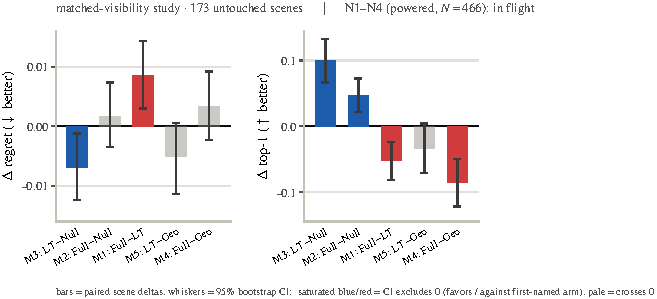
\includegraphics[width=\linewidth]{figs/fig_results.pdf}
  \caption{\textbf{All primary contrasts} ($K{=}8$ selected regret left, tie-aware top-1 right; bars are paired scene deltas, whiskers 95\% bootstrap CIs, drawn directly from the locked analysis records). Saturated blue/red: CI excludes zero, favoring / opposing the first-named arm; pale gray: CI crosses zero. M1--M5: matched-visibility study; N1--N4: powered incumbent study.}
  \label{fig:results}
\end{figure}

\subsection{Effectiveness of the Frozen Last Token}
\label{sec:res-signal}

The paired contrast that isolates scene information, \Ltok{} versus the graph- and parameter-identical scene-blind \Lnull, is supported on both co-primary endpoints: selected regret $-0.0069$ and top-1 agreement $+0.100$, both CIs excluding zero (\cref{tab:main}, M3), on scenes no model in the study had ever consumed.
In absolute terms \headname{} recovers regret from $0.0439$ to $0.0371$ and lifts top-1 agreement from $0.567$ to $0.667$ (\cref{tab:main-abs}); secondary endpoints agree, with pairwise ranking accuracy $+0.068$ and top-1 $+0.083$ at $K{=}5$ and $+0.046$ at $K{=}2$, all CIs excluding zero.
The effect replicates the direction and magnitude first observed on development scenes during the design phase, making this its first prospective confirmation on an untouched cohort.\TODO{supp: add the development-phase (E1) record values as the internal-replication table}

Dependence on scene content, not merely on the presence of some input, is established by inference-time ablations on the sequence-reading arm (\cref{fig:ablations}): substituting a different scene's representation degrades top-1 by $0.019$ and zeroing it by $0.024$, both CIs excluding zero, while regret shifts stay small ($+0.0007$ and $+0.0012$, CIs crossing zero) with no contradictory material improvement on either endpoint.
The degradation concentrating on top-1 is the expected signature: scene content is what disambiguates near-tied candidates at the top of the list.
The full-sequence arm corroborates the signal's existence from a second angle: \Lfull{} also beats \Lnull{} on top-1 ($+0.047$, CI excluding zero; \cref{tab:main}, M2), so the sequence contains the information, which sharpens the next finding: the failure of \Lfull{} is about form, not existence.

\begin{figure}[t]
  \centering
  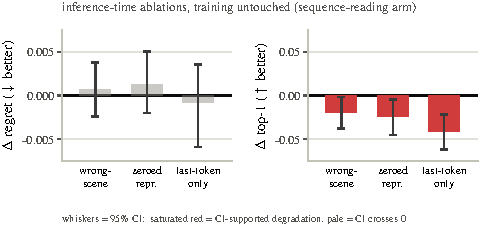
\includegraphics[width=\linewidth]{figs/fig_ablations.pdf}
  \caption{\textbf{Causal ablations} (inference-time, training untouched; deltas versus the arm's NORMAL condition at $K{=}8$, 95\% CIs). Wrong-scene substitution and zeroing degrade top-1 (CIs exclude zero); the last-token-only diagnostic degrades the \Lfull{} reader (top-1 $-0.041$, CI excluding zero), showing it genuinely consumes sequence positions, yet it still loses to the last-token-trained arm end-to-end (\cref{sec:res-onetoken}).}
  \label{fig:ablations}
\end{figure}

\subsection{Last Token versus Full Sequence}
\label{sec:res-onetoken}

Giving the reader the entire $3{,}086\times4{,}096$ prefill, strictly more information than its last row under an identical parameter budget (1{,}708{,}871 parameters, interchangeable state dicts), makes the audit worse, with support on both primaries: regret $+0.0085$ and top-1 $-0.053$, both CIs excluding zero (\cref{tab:main}, M1).
The deficit is consistent, not a $K{=}8$ artifact: top-1 $-0.037$ at $K{=}5$ and $-0.021$ at $K{=}2$, pairwise accuracy $-0.033$; no CI extends above zero.

Two probes localize the mechanism.
First, the \Lfull{} reader did not degenerate into a last-token reader: feeding it only the final row at inference costs it a further $0.041$ top-1 (CI excluding zero; \cref{fig:ablations}), so it genuinely attends across the sequence.
The cost is therefore paid at training time: spreading a fixed-capacity reader's cross-attention over 3{,}086 tokens yields a worse audit function than concentrating it on the one token where the generator has already aggregated the scene, the state from which it began emitting candidates.
Second, the auxiliary consequence heads split: \Lfull{} is worse on future-trajectory ADE ($+0.021$) and collision AUROC ($-0.137$; $n{=}29$ scenes with defined labels) but better on FDE ($-0.072$), each CI excluding zero.
Sequence access is not uniformly useless, since it helps some long-horizon geometry, but the audit-relevant summary is best read where the generator itself deposited it.
Under matched parameters, explanations based on reader capacity are excluded by design; what remains is information accessibility.
For practitioners the implication is direct: the cheapest representation (one token, $47\times$ less memory than the sequence; \cref{sec:res-eff}) is also the right one.

\subsection{Comparison with a Trained Geometric Auditor}
\label{sec:res-incumbent}

Against the trained geometry incumbent, the matched-visibility study ends in tension (\cref{tab:main}, M5): \headname{} leads on regret ($-0.0051$) while the incumbent leads on top-1 agreement ($-0.033$; absolute levels $0.700$ versus $0.667$), and both CIs cross zero.
At $N{=}173$ this comparison is underpowered for the observed effect; concluding either way would be exactly the practice the protocol is designed to prevent.
We therefore preregistered a consolidation study sized for it: $N=466$ scenes gives $1-\beta=0.800$ at two-sided $\alpha=0.05$ for the locked MDE ($0.00514$ regret), with all arms, gates, margins, nomination order, and analysis code frozen before any new scene was scored.

On 525 scenes, neither candidate displaces the incumbent.
Against \Lgeo, the checkpoint-objective candidate lands at regret $-0.0014$ and top-1 $+0.003$, the selector-objective candidate at $+0.0016$ and $+0.003$; all four CIs cross zero (\cref{tab:main}, N1 and N1$'$).
Both fail the preregistered regret-superiority gate (G1) and the robustness gate (G8), and the selector-objective candidate additionally fails the selector-trade gate (G5); no arm is nominated and the sealed cohort stays sealed.
The scene-value contrast, by contrast, replicates at scale and is the strongest of the program: N2 regret $-0.0129$ and top-1 $+0.112$ over the scene-blind control, both CIs excluding zero by a wide margin (\cref{tab:main}).
We report this as a boundary result with unusual evidential value: at $0.80$ power, the frozen representation demonstrably adds scene information a geometry auditor lacks, yet that information is not sufficient to beat a well-tuned geometric baseline on the promoting endpoint at the effect size that motivated the study.
Representation reuse pays when no tuned incumbent exists or when top-of-list disambiguation, where the scene signal concentrates, is the binding constraint; it does not automatically retire strong geometric priors.

\subsection{Effect of the Selector Loss}
\label{sec:res-selloss}

The controlled contrast N3 isolates the objective of \cref{eq:selloss}: same architecture, same data, rank term replaced by the regret-weighted best-vs-rest logistic.
The preregistered success criterion is asymmetric by design: the selector loss must buy top-1 (CI above zero) without selling regret (CI upper bound below $+0.005$), because the design-phase precedent showed a large top-1 gain at a small regret concession.\TODO{supp: cite exact E1 record values}

N3 lands at top-1 $-0.000$ (CI crossing zero) and regret $+0.0029$ (CI excluding zero; \cref{tab:main}): the selector loss buys no top-1 on the enlarged cohort and sells regret with CI support, so the trade does not clear the gate.
The top-of-list gain seen in the design phase did not survive prospective replication at scale; we retain the checkpoint objective as the reference configuration.

\subsection{Deployment Cost}
\label{sec:res-eff}

\Cref{tab:eff} summarizes deployment cost on a single workstation GPU.
The deployed configuration, last token in and all $K{=}8$ candidates scored, runs in $1.19$\,ms median ($1.21$\,ms p95) with $3.5$\,MB peak incremental memory and 1{,}708{,}871 trainable parameters, orders of magnitude under the preregistered ceilings ($10$/$15$\,ms, $1$\,GiB, 2{,}000{,}000 parameters).
The representation itself is free: it is a byproduct of the prefill that generates the candidates.
No VLA finetuning, no world model, no inference-time rollouts; the entire auditor trains in minutes (peak $398.7$\,MB per worker).
For contrast, the full-sequence reader needs $165.2$\,MB at inference ($47\times$ more) and is worse (\cref{sec:res-onetoken}); explicit-imagination designs additionally pay for a purpose-trained world model and its inference-time rollouts, a cost class our zero-rollout route avoids entirely.

\begin{table}[t]
  \centering
  \small
  \setlength{\tabcolsep}{4pt}
  \begin{tabular}{@{}lrrr@{}}
    \toprule
    & Params & Latency (ms) & Peak mem \\
    \midrule
    \Ltok{} (ours) & 1{,}708{,}871 & $1.19$\,/\,$1.21$ & $3.5$\,MB \\
    \Lfull{} (sequence) & 1{,}708{,}871 & $1.29$\,/\,$1.30$ & $165.2$\,MB \\
    \midrule
    Preregistered ceiling & 2{,}000{,}000 & $10$\,/\,$15$ & $1$\,GiB \\
    \bottomrule
  \end{tabular}
  \caption{\textbf{Deployment cost} (incremental over the generator, all $K{=}8$ candidates, bf16, single workstation GPU). \Ltok{} is the deployed configuration; latency is median\,/\,p95 over 200 timed iterations.}
  \label{tab:eff}
\end{table}
